\documentclass[10pt]{article}
\usepackage[margin=.76in]{geometry}
\usepackage{amsmath,amssymb,booktabs,microtype,enumitem,hyperref,graphicx,float}
\usepackage[T1]{fontenc}\usepackage{lmodern}
\setlist{nosep,leftmargin=*}
\hypersetup{colorlinks=true,linkcolor=blue,urlcolor=blue,hypertexnames=false}
\title{Autoregressive Inference Before Tools:\\The Multi-Token Computational Frontier of Tiny Transformers}
\author{Paper 0.85 --- Multi-Token Inference Research Line}
\date{Stage-1 and recurrence-frontier results --- September 2026}
\begin{document}\maketitle
\begin{abstract}
A one-token Transformer is a fixed-depth circuit, but a decoder generating multiple tokens is already an iterative machine: each generated token becomes writable state, and subsequent steps can attend to the full trajectory. Before attributing systematic reasoning gains to external agents or tools, we measure how much computation ordinary autoregressive generation learns by itself. A leakage-audited local gate first establishes one-step implication over held-out ordered pairs with shared, fully trained lexical support: all three L2/W64/H4 seeds exceed 98.8\% on positive and negative controls. We then train proof chains only at $K\le3$. One-token answers (O0), free traces (O1), and fully teacher-forced structured traces (O3) reach a three-seed frontier of three but fail abruptly at the first unseen depth. A second, token-matched 12-run O1 experiment tests random partial starts, higher chain diversity, and their combination. Every condition again has stable $K_{\rm AR}=3$ and $P_{\rm acquire}(K=4)=0/3$; partial-start conditions fail mainly by premature termination. Correct-prefix injection does not rescue the original $K=4$ failures and instead exposes strong absolute-step dependence. Thus recurrence is constructively representable (Paper 0.1) but is not acquired under these recurrence-targeted curricula. This is bounded evidence against reusable learned recurrence in the tested regime, not evidence against autoregressive expressivity or a claim of mathematical non-closure.
\end{abstract}

\section{Motivation}
Suppose the context contains
\[
A,\quad A\Rightarrow B,\quad B\Rightarrow C,\quad C\Rightarrow D.
\]
A one-token answer to query $D?$ requires internal composition before output. An autoregressive model can instead emit
\[
A\rightarrow B\rightarrow C\rightarrow D
\]
or a structured trajectory such as
\[
KNOWN(A),\ DERIVE(B),\ DERIVE(C),\ DERIVE(D),\ ANSWER(TRUE).
\]
The model weights are unchanged, but the effective machine is not. Generated tokens form external state:
\[
s_{t+1}=F_\theta(X,s_{\le t}).
\]
Paper 0.85 isolates this resource before adding tools.

\section{Scope}
The first version uses deliberately simple propositional implication. More complex single-step syntax---negation, conjunction, variables, predicates, functors, frames, algebraic rewrites---should only be added after Paper 0.7 establishes which local operators are reliably learned.

The primary question is therefore:
\[
\boxed{\text{given a reliably learned local implication step, can autoregression learn reusable proof recurrence?}}
\]

\section{Task prerequisite}
Every recurrence experiment first passes a local-step gate:
\[
A,\quad A\Rightarrow B\vdash B.
\]
A model that cannot reliably solve this across held-out proposition pairs cannot support an interpretable closure experiment. Report $P_{\rm acquire}^{\rm local}$ across model and generator seeds, while ensuring that lexical output support is not accidentally withheld.

R0-v1 withheld proposition identities entirely. Its three seeds learn the negative label (98.8--99.6\%) but achieve only 4.3--6.6\% entailed accuracy and 4.7--7.8\% on consequent swaps despite near-zero training loss. Because held-out symbols also have untrained output rows, this is a useful lexical/OOV-output transfer stress, not the central implication gate.

R0-v2 corrects that confound. All 64 symbols occur during training as inputs and positive targets; 3,226 ordered implication pairs train the model and 806 pairs are held out, with zero observed pair leakage. Entailed, consequent-swap, fact-mismatch, and rule-LHS-mismatch controls are balanced. At L2/W64/H4, seed 11 scores 100\% on all four conditions; seed 23 scores 100\%, 100\%, 100\%, and 99.6\%; seed 37 scores 98.8\%, 98.8\%, 99.6\%, and 100\%. The preregistered 95\% three-seed gate therefore passes. This establishes local implication over held-out pairs with trained lexical support; it does not establish recurrence.

\section{Dataset ladder}
\subsection{R0: direct one-step implication}
Use arbitrary proposition symbols and disjoint train/test identities where feasible.

\subsection{R1: fixed two-step chains}
\[
A,\ A\Rightarrow B,\ B\Rightarrow C\vdash C.
\]
Train both direct-answer and derivation-output conditions.

\subsection{R2: variable chain length}
Generate
\[
A_0,\quad A_0\Rightarrow A_1,\ldots,A_{K-1}\Rightarrow A_K.
\]
Train $K\le K_{\rm train}$, initially $K_{\rm train}\in\{2,3\}$. Test
\[
K\in\{1,2,3,4,6,8,12,16,24,32,64\}.
\]

\subsection{R3: shuffled rule order}
Randomize implication order to remove a trivial left-to-right copying strategy.

\subsection{R4: distractor rules}
Add irrelevant implications with
\[
N\in\{0,2,4,8,16,32,64\}.
\]

\subsection{R5: branching}
Introduce multiple outgoing rules and competing branches only after chain recurrence works. Keep a unique target proof initially, then increase search ambiguity.

\subsection{Executable generator and split contract}
The broad CPU instrument stores the fact, ordered ground-truth chain, implication multiset, query, minimal proof depth, distractor count, branching factor, shuffle flag, split, and split-specific namespace. Branches terminate away from the query, so the target proof remains unique; distractor antecedents are unreachable from the initial fact. The exact validator checks every chain edge, namespace membership, and target-path uniqueness before serialization.

The full CPU materialization contains 2,800 examples. Training is strictly bounded to $K\in\{1,2,3\}$; validation and test cover all eleven preregistered depths. All splits cross seven distractor levels, ordered/shuffled presentations, and branching factors one/two. Every row passes the symbolic validator. Four exact target serializations per example produce 11,200 reference traces. These reference outputs pass exact trajectory checks and are labeled \texttt{reference\_oracle}; they establish generator correctness, not model performance.

The learned Stage-1 instrument uses the R0-v2 shared vocabulary and partitions ordered implication edges rather than lexical identities. Every edge in a training chain belongs to the training pair set and every evaluation edge belongs to the held-out pair set; observed edge leakage is zero. The query is a bare instruction token and contains no answer argument. This last audit was added after an initial pilot serialized \texttt{QUERY target}, producing a trivial copy path. That pilot is quarantined as invalid and contributes no result or figure.

\section{Output-machine conditions}
\paragraph{O0: one-token answer.} Emit final conclusion/boolean only.
\paragraph{O1: free multi-token generation.} Train an untyped proposition trace and score final answer, transitions, exact trajectory, and termination.
\paragraph{O2: structured scratchpad without state labels.} Supervise grammar/control tokens and the final answer, but withhold intermediate proposition labels. Use minimal tokens such as
\[
\langle STATE:A\rangle\langle DERIVE:B\rangle\cdots\langle ANSWER:D\rangle.
\]
No external semantic operation is executed.
\paragraph{O3: teacher-forced derivation training.} Supervise every structured intermediate proof token in training, then autoregress at test. The O2--O3 contrast isolates intermediate semantic supervision from format supervision; neither condition executes an external operation.

\section{Core recurrence hypothesis}
A learned proof procedure should approximate
\[
s_t=\text{current known proposition},
\]
\[
s_{t+1}=\operatorname{NextApplicableRule}(s_t,\mathcal R).
\]
For a pure chain this transition is local and time-invariant. If acquired, larger test proof depth should primarily increase generated steps rather than require a larger network.

\section{Internal versus autoregressive composition}
Define
\[
K_{\rm internal}(M)
\]
as the largest one-token chain length meeting the competence gate, and
\[
K_{\rm AR}(M)
\]
as the largest multi-token chain length meeting the same final-answer gate. Primary difference:
\[
G_{\rm recurrence}=K_{\rm AR}-K_{\rm internal}.
\]
Report full curves, not only maxima.

\section{Corrected Stage-1 results}
The first learned comparison fixes the passing R0-v2 architecture (L2/W64/H4), uses 1,000 updates per cell, trains only at $K\in\{1,2,3\}$, and evaluates 64 held-out-pair chains at each $K\in\{1,2,3,4,6,8\}$ for seeds 11, 23, and 37. Competence requires at least 95\% final and termination accuracy for every seed. Table~\ref{tab:frontier} reports only measured points.

\begin{table}[H]\centering\small
\begin{tabular}{llll}
\toprule
Condition & Supervision & Three-seed frontier & $P_{\rm acquire}(K=4)$\\\midrule
O0 & final answer & 3 & 0/3\\
O1 & free proposition trace & 3 & 0/3\\
O2 & structure+final, no states & none & 0/3\\
O3 & full structured trace & 3 & 0/3\\
\bottomrule
\end{tabular}
\caption{Leakage-free Stage-1 frontiers. ``None'' means that O2 fails the gate even in range; it does not mean that the model produces no correct tokens.}\label{tab:frontier}
\end{table}

O0 is 100\% for all seeds at $K=1,2,3$, then falls at $K=4$ to 0\%, 1.6\%, and 4.7\%. O1 is likewise perfect in range but reaches only 1.6\%, 1.6\%, and 0\% at $K=4$. Its transition accuracy at that boundary is 32.0\%, 32.0\%, and 23.4\%; at $K=6,8$ it falls to roughly 10--20\%. Termination, perfect in range, becomes seed- and depth-dependent out of range. Free generation therefore adds writable tokens but does not acquire a reusable transition in this regime.

O2 separates syntax from semantics. Across depths its seed-level aggregate final accuracy is 9.1\%, 25.0\%, and 3.4\%; transition accuracy is 1.3--4.6\%, and no exact trajectory occurs, although termination can remain high. The model learns much of the requested output grammar without the missing state labels. O3 restores perfect in-range trajectories, yet at $K=4$ final accuracy is only 1.6\%, 0\%, and 0\%; deeper values remain near chance. Richer derivation supervision improves interpolation but does not create extrapolative recurrence.

\begin{figure}[H]\centering
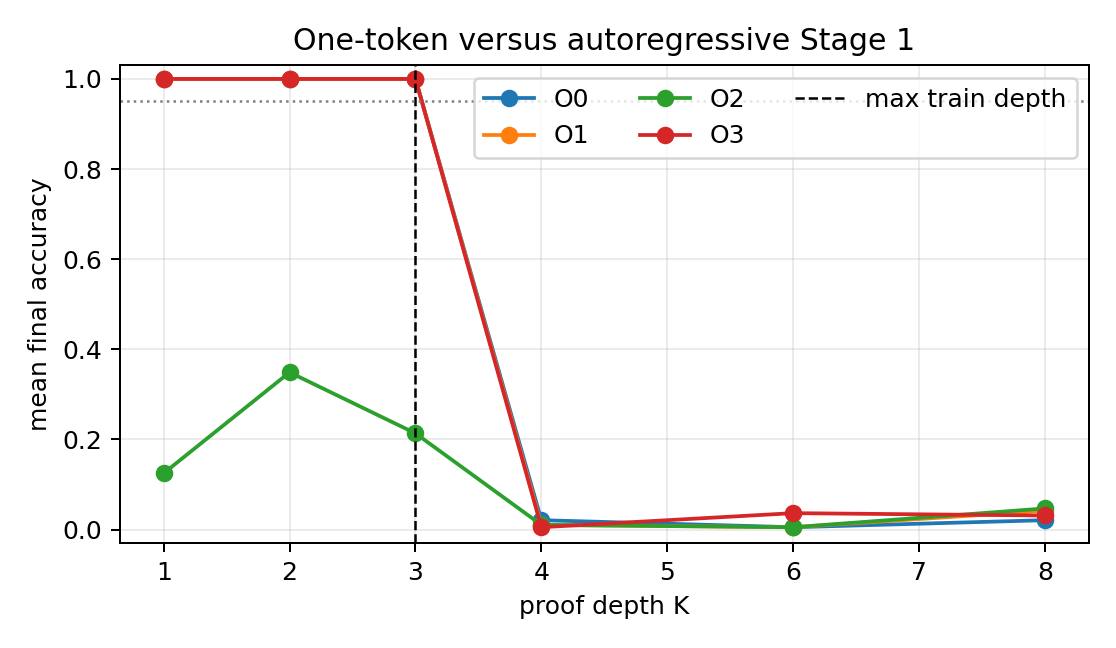
\includegraphics[width=.72\linewidth]{../paper0_85/results/recurrence_stage1_v2/figures/one_token_vs_multitoken_depth.png}
\caption{Mean three-seed final accuracy for the corrected Stage-1 comparison. The dashed line marks the maximum training depth. The sharp shared boundary, rather than gradual accumulated error, provides no evidence for reusable recurrence beyond the training range.}
\end{figure}

Consequently,
\[
K_{\rm internal}=K_{\rm AR}=K_{\rm O3}=3,
\qquad G_{\rm recurrence}=0
\]
over the tested architecture, supervision, and depths. This is a finite empirical statement. It neither proves that autoregression cannot expand the frontier under another curriculum/architecture nor licenses infinite-closure claims.

\section{What changes the recurrence frontier?}
\subsection{Matched intervention design}
The next iteration tests whether the original solution is bound to complete-trajectory starts or to repeated chain templates. We retain O1, L2/W64/H4, seeds 11/23/37, 1,000 updates, and $K_{\rm train}\le3$, and evaluate the same 64 held-out-pair chains per seed at $K\in\{1,2,3,4,5,6,8\}$. Four conditions cross complete versus random partial starts with ordinary versus nonrepeating high-diversity sampling. Partial examples begin at internal states of latent chains with depth 4, 5, 6, or 8 while exposing only residual lengths 1--3; complete starts remain in the mixture. High-diversity sampling prevents repeats for depth above one, where the finite depth-one pair set must repeat.

Every condition processes exactly 96,000 examples and 4,512,000 fixed-padded causal positions per seed. Deterministic sampling audits find mean distinct latent-chain counts of 42,752 (baseline), 53,823 (partial starts), 44,094 (high diversity), and 54,198 (partial plus diversity); all conditions cover all 3,226 training transitions. Thus the intervention changes start-position and chain-repetition statistics under matched optimizer exposure, but the fresh-online baseline is already diverse. The labels ``high diversity'' and ``partial starts'' name sampling policies, not assumptions that they must improve generalization.

\subsection{Frontier and failure results}
\begin{table}[H]\centering\small
\begin{tabular}{lcccc}
\toprule
O1 condition & Seed frontiers & Stable $K_{\rm AR}$ & $P_{\rm acquire}(K=4)$ & Mean $K=4$ transition\\\midrule
Baseline & 3/3/3 & 3 & 0/3 & .305\\
Partial starts & 3/3/3 & 3 & 0/3 & .008\\
High diversity & 3/3/3 & 3 & 0/3 & .305\\
Partial starts + diversity & 3/3/3 & 3 & 0/3 & .003\\
\bottomrule
\end{tabular}
\caption{Corrected recurrence-frontier experiment. A frontier is the largest contiguous depth passing final $\ge.95$, termination $\ge.95$, and exact trajectory $\ge.90$ in that seed; the stable frontier is the minimum across seeds.}
\label{tab:recurrence-v2}
\end{table}

All 12 cells remain competent through the training range, but every condition has zero final accuracy at $K=4$. High diversity leaves the boundary transition mean numerically unchanged at .305. Partial starts do not merely fail to rescue extrapolation: at $K=4$ their mean transition accuracy is .008 without the diversity constraint and .003 with it. Both partial-start conditions terminate prematurely on every boundary example, whereas baseline and high-diversity conditions mostly terminate late (mean delayed-termination rates .844 and .771). These distinct failure modes show that endpoint collapse alone is not a sufficient mechanism description. They do not show that partial starts are intrinsically harmful: this particular mixture may strengthen a learned residual-length stop policy, and no curriculum-weight or explicit termination objective was varied.

\begin{figure}[H]\centering
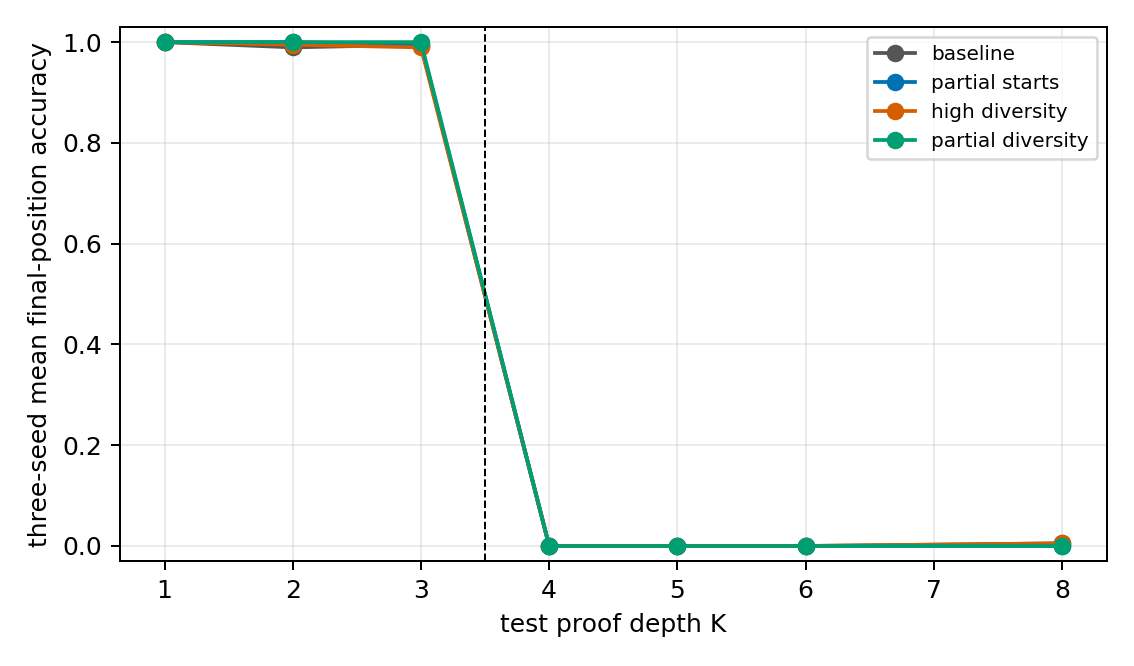
\includegraphics[width=.49\linewidth]{../paper0_85/results/recurrence_frontier_v2/frontier_by_condition.png}\hfill
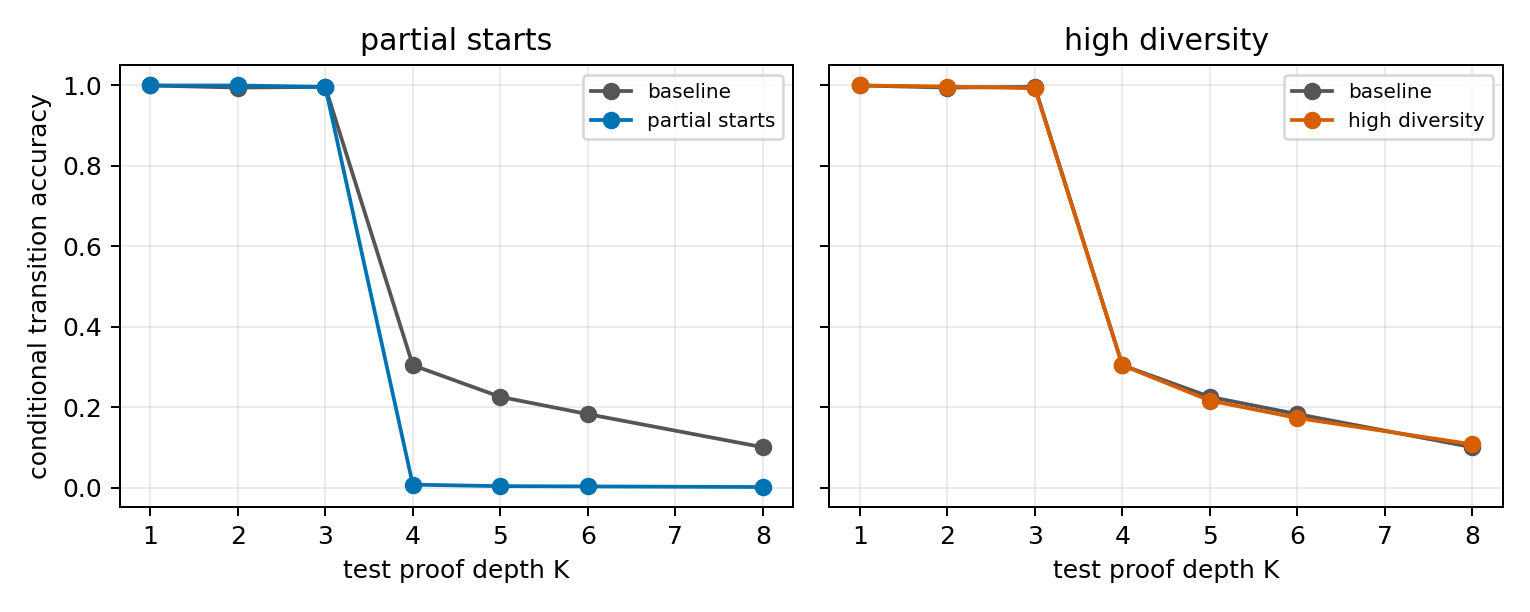
\includegraphics[width=.49\linewidth]{../paper0_85/results/recurrence_frontier_v2/intervention_transition_accuracy.png}
\caption{Three-seed O1 results under matched training exposure. Left: every condition crosses the training boundary at $K=3\to4$. Right: partial-start conditions sharply reduce conditional transition accuracy out of range; enforced diversity alone closely tracks baseline. Dashed vertical position marks the first unseen depth.}
\label{fig:recurrence-v2}
\end{figure}

\subsection{Oracle-prefix diagnostic}
To distinguish accumulated early errors from an absolute-step failure, we evaluate the original corrected Stage-1 O1 checkpoints on $K=4$ while injecting proper target prefixes of length zero through three. The final answer is never included in a forced prefix, the query contains no answer field, and evaluation uses held-out implication pairs. With no injection, the first next state is correct on .964 of examples on average, yet the remaining trajectory is never exact. After forcing one, two, and three correct states, accuracy on the next required state falls to .146, .099, and .005; final accuracy remains zero except .005 at prefix length three. Termination accuracy stays between .010 and .036.

\begin{figure}[H]\centering
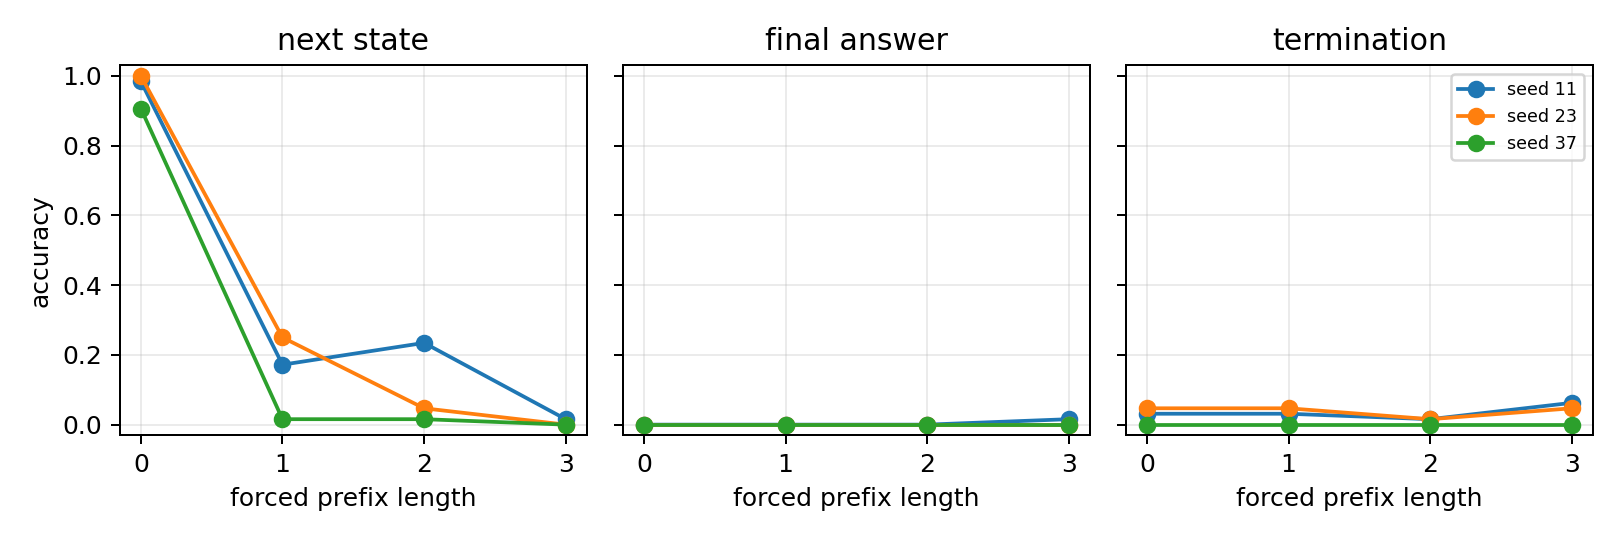
\includegraphics[width=.58\linewidth]{../paper0_85/results/recurrence_frontier_v2/oracle_prefix/oracle_prefix_rescue.png}
\caption{Leakage-audited oracle-prefix diagnostic at $K=4$ (three seeds, 64 examples each). Correct prefixes do not rescue continuation; performance worsens as the required prediction moves to a later absolute output position.}
\label{fig:oracle-prefix}
\end{figure}

The diagnostic argues against ordinary error propagation as the main explanation for the sharp boundary. It is consistent with an absolute-step or total-length template: the first local move is usually available, but the same semantic move is not reused at later generated positions even after the preceding state is supplied correctly. Because absolute step and remaining total length are not independently randomized in this diagnostic, it does not identify which cue controls the failure.

The preregistered gate for a matched O0 follow-up required an O1 condition to reach unseen $K\ge4$; no condition did, so that follow-up was not opened. Accordingly this iteration does not change $K_{\rm internal}$ or establish $G_{\rm recurrence}>0$. It strengthens the narrower conclusion: a reusable fixed-weight recurrence exists constructively in Paper 0.1, while SGD here acquires a bounded trajectory policy even after two targeted data interventions.

\section{Closure signatures}
Train on $K\le2$ or $3$ and test much larger $K$. Evidence for reusable recurrence strengthens when:
\begin{enumerate}
\item accuracy remains high far beyond $K_{\rm train}$;
\item generated step count scales with true proof depth;
\item the same local transition is used at early and late steps;
\item state representations align by proof role rather than absolute generation index;
\item failure depends mainly on accumulated local error or context budget rather than a sharp learned maximum length.
\end{enumerate}
Do not claim literal $K=\infty$ closure from finite tests.

\section{Finite-context versus idealized closure}
Let $C_{\max}$ be context capacity. Even a correct recurrence eventually fails if its serialized trajectory exceeds available memory. Report $K_{\rm AR}(M,C_{\max})$ and distinguish procedure failure from context overflow.

\section{Acquisition probability}
For architecture $M$ and training distribution $\mathcal D$ define
\[
P_{\rm acquire}^{\rm recurrence}=P_s[A(K_{\rm test}\gg K_{\rm train})\ge\gamma].
\]
Distinguish recurrence representable but rarely acquired, recurrence reliably acquired, and local rule acquired but recurrence not acquired.

\section{Architecture grid}
Start with
\[
L\in\{1,2,3,4\},\quad W\in\{16,32,64\},\quad H\in\{1,2,4\},
\]
and training budgets $T\in\{1,2,4\}\times$. This diagnostic grid, four output conditions, and three model seeds enumerates 1,296 possible phase cells, not completed evidence. Stage 1 runs only the 12-cell passing R0 architecture slice, and the recurrence-frontier iteration adds 12 O1 data-intervention cells at the same architecture. Deeper $L\in\{6,8\}$ and wider $W=128$ cells remain conditional expansions. The next discriminating experiment is local next-state/termination supervision or a $K_{\rm train}^{\max}=4$ transfer test, not a broad architecture sweep.

\section{Mechanistic measurements}
At every generation step record next-token distribution, correct-next-state rank/margin, Q/K/V, attention role mass, SA/FF residual increments, representation similarity across recurrence steps, and attention to original rules versus generated state.

For correct next state $s_{t+1}^*$ define
\[
m_t=z_t(s_{t+1}^*)-\max_{y\ne s_{t+1}^*}z_t(y).
\]
Test whether $m_t$ degrades with absolute step index after controlling local-rule difficulty.

\section{Causal tests}
For competent recurrent models:
\begin{itemize}
\item patch a same-role state from another proof depth;
\item replace an intermediate proposition with correct/incorrect alternatives;
\item mask previous proof states while preserving original rules;
\item mask original rules after they are supposedly encoded into generated state;
\item ablate heads/FF components by recurrence step;
\item compare same-role transitions across unseen proposition identities.
\end{itemize}
A genuine recurrence should be more invariant to absolute step number than a memorized fixed-length trajectory.

\section{Error accumulation and termination}
Estimate conditional transition accuracy
\[
p_t=P(s_{t+1}\text{ correct}\mid s_{\le t}\text{ correct}).
\]
Compare whole-proof accuracy with $\prod_t p_t$ as a simple independent-error baseline. Analyze premature answer, failure to terminate, trajectory drift, wrong applicable rule, and context overflow separately.

Under the deliberately restrictive baseline that transitions are independent conditional on a correct prefix and $p_t=p$, whole-proof success is $p^K$. The experiment must compare observed success against $\prod_t p_t$, because attention to the full generated history permits correlated errors and self-repair. A positive or negative deviation is therefore a diagnostic of dependence, not automatically evidence for or against recurrence.

\section{CPU-validated serialization frontier}
The prompt token count in the pure ordered chain is $4K+6$ under the whitespace audit tokenizer. O0 adds one target token, O1 adds $K+1$, and O2/O3 add $2K+5$. At $K=64$, the resulting audited totals are 263, 327, and 395 tokens, respectively. These values provide exact context-budget denominators for the present serialization; tokenizer-specific model runs must also report their true subword lengths.

\begin{figure}[H]\centering
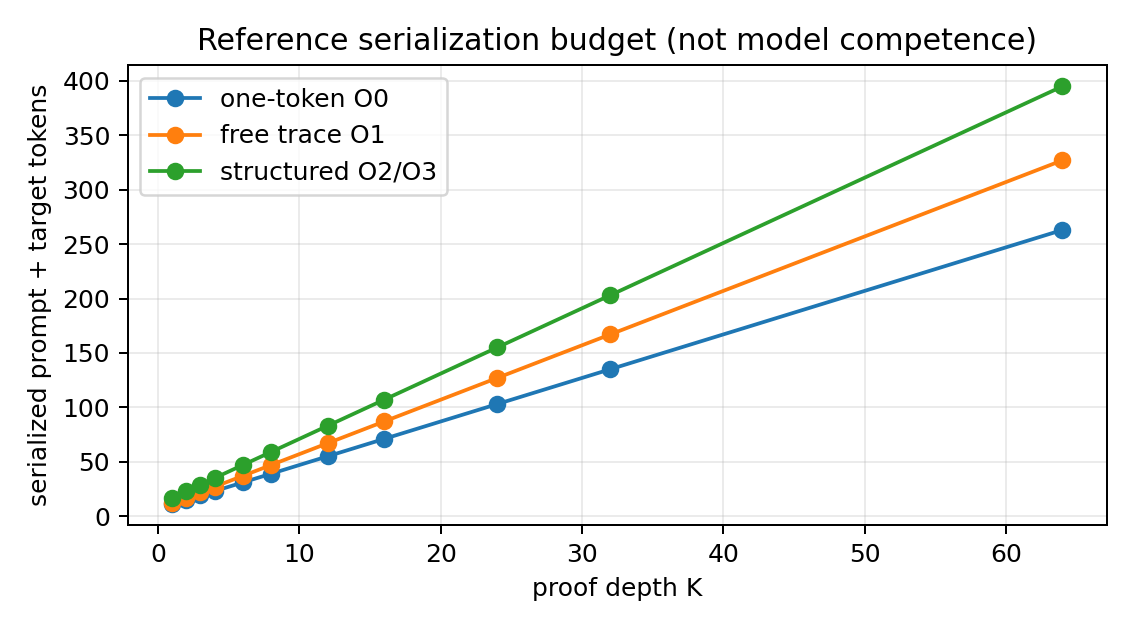
\includegraphics[width=.68\linewidth]{../paper0_85/results/figures/context_budget_frontier.png}
\caption{Prompt-plus-target length for the validated reference serialization. This is a dataset geometry result, not a learned competence frontier.}
\end{figure}

The learned Stage-1 results above report accuracy, measured frontiers, transition accuracy, and termination. Role invariance and causal recurrence tests remain blocked because no condition is recurrently competent beyond the training range. Exact oracle performance is never entered into a model-results table.

\section{ICL extension}
After base recurrence is understood, compare rules learned in weights against novel implication graphs supplied entirely in context with held-out symbols. If the latter succeeds at long depth, the clean interpretation is:
\[
\text{context supplies instance-specific facts/rules}+\text{weights supply recurrence procedure}.
\]
Do not add this extension before a stable recurrence regime exists.

\section{Relation to Papers 0.7 and 0.9}
Paper 0.7 measures one-pass formal computation. Paper 0.85 adds self-generated intermediate state. Paper 0.9 adds deterministic external operations and an explicit loop. The required ladder is
\[
\boxed{\text{one-token}\to\text{free multi-token}\to\text{structured scratchpad}\to\text{tool/harness}.}
\]
Only this can distinguish class expansion from improved learnability/reliability.

\section{Contribution and remaining question}
The present negative result combines reliable local implication, a three-seed train-short/test-long boundary, two recurrence-targeted data interventions, and a leakage-audited prefix diagnostic. It locates a learned boundary between having autoregressive writable state and acquiring a transition that reuses it systematically. It does not reduce the theoretical expressivity of autoregressive Transformers: Paper 0.1's handcrafted fixed-weight witness supplies the relevant representability contrast. The remaining question is which supervision or curriculum, if any, produces $K_{\rm AR}>K_{\rm internal}$ under a matched model and budget.

\section{Reproducibility and evidence status}
The executable components are:
\begin{itemize}
\item generator/evaluator: \path{src/cl/semantic/autoregressive_proofs.py};
\item phase materialization: \path{src/cl/experiments/paper085_phase.py};
\item serialization analysis: \path{src/cl/experiments/paper085_analyze.py};
\item configuration: \path{configs/paper085/phase_v1.json}.
\item R0-v2 gate: \path{paper085_r0_gate_v2.py} with \path{r0_gate_v2.json};
\item recurrence runner: \path{paper085_recurrence_stage1.py};
\item recurrence analysis: \path{paper085_recurrence_analyze.py};
\item recurrence configuration: \path{recurrence_stage1_v2.json}.
\item recurrence-frontier runner: \path{paper085_recurrence_frontier_v2.py};
\item recurrence-frontier analysis: \path{paper085_recurrence_frontier_analyze_v2.py};
\item recurrence-frontier configuration: \path{recurrence_frontier_v2.json}.
\end{itemize}
Machine-readable artifacts are under \path{docs/papers/paper0_85/results}. The authoritative second-iteration aggregate contains exactly 84 condition--seed--depth cells and 12 sampling-audit cells; its manifest records the four conditions, three-seed completeness, matched 4,512,000-position budget, and closed O0 follow-up gate. The broad phase manifest explicitly labels its 11,200 exact traces as reference results rather than learned evidence. Learned R0-v1, R0-v2, corrected Stage1-v2, and recurrence-frontier-v2 occupy isolated directories; Stage1-v1 is quarantined because of query-target leakage. The recurrence-frontier \path{smoke/} and \path{invalid_low_diversity_baseline/} directories are explicitly excluded from aggregation, as are superseded pilot designs. Tracked dense checkpoints are locally reproducible and may remain ignored. Planned context-limit, role-invariance, causal, shuffled-rule, distractor, branching, and ICL experiments are not stated as findings.

\begin{thebibliography}{99}
\bibitem{li2024} Z. Li, H. Liu, D. Zhou, and T. Ma. Chain of Thought Empowers Transformers to Solve Inherently Serial Problems. arXiv:2402.12875, 2024.
\bibitem{joshi2025} N. Joshi et al. A Theory of Learning with Autoregressive Chain of Thought. \emph{COLT}, 2025.
\bibitem{bavandpour2025} A. A. Bavandpour et al. Lower Bounds for Chain-of-Thought Reasoning in Hard-Attention Transformers. \emph{ICML}, 2025.
\end{thebibliography}
\end{document}
